\chapter{Extended Design Space Surface Maps}
\label{Appendix: Supplementary Surface Maps}

\par This appendix collects the surface maps that were computed by the design space exploration of Chapter \ref{chapter: methodology} but were not reproduced in the main text. They are provided for completeness and to support the validation of the design strategy during the first experimental campaign.

\section{Pixel density and in-focus field of view}
\label{section: Appendix pixel density}

\par Figure \ref{fig: Px pitch and LFOV surfmap SBOS} displays the pixel density $\rho_{px}$ and the field of view of the in-focus plane $L_{FoV}$ for the negative defocus setup of Section \ref{subsection: Surface Maps for SBOS}. Both quantities depend only on the optical magnification, through Equation \ref{equation: Px density} and $L_{FoV} = L_{sens}/M_{ag}$, so they present the same trends as $M_{ag}$ in Figure \ref{fig: M,m and df design surfmap SBOS}. The pixel density increases with $l$ and decreases with $f$, while $L_{FoV}$ shows the inverse behavior. The in-focus plane is where the calibration plate is positioned, therefore these maps can be directly compared to the measured values during the experimental campaign.

\begin{figure}[htbp]
    \centering
    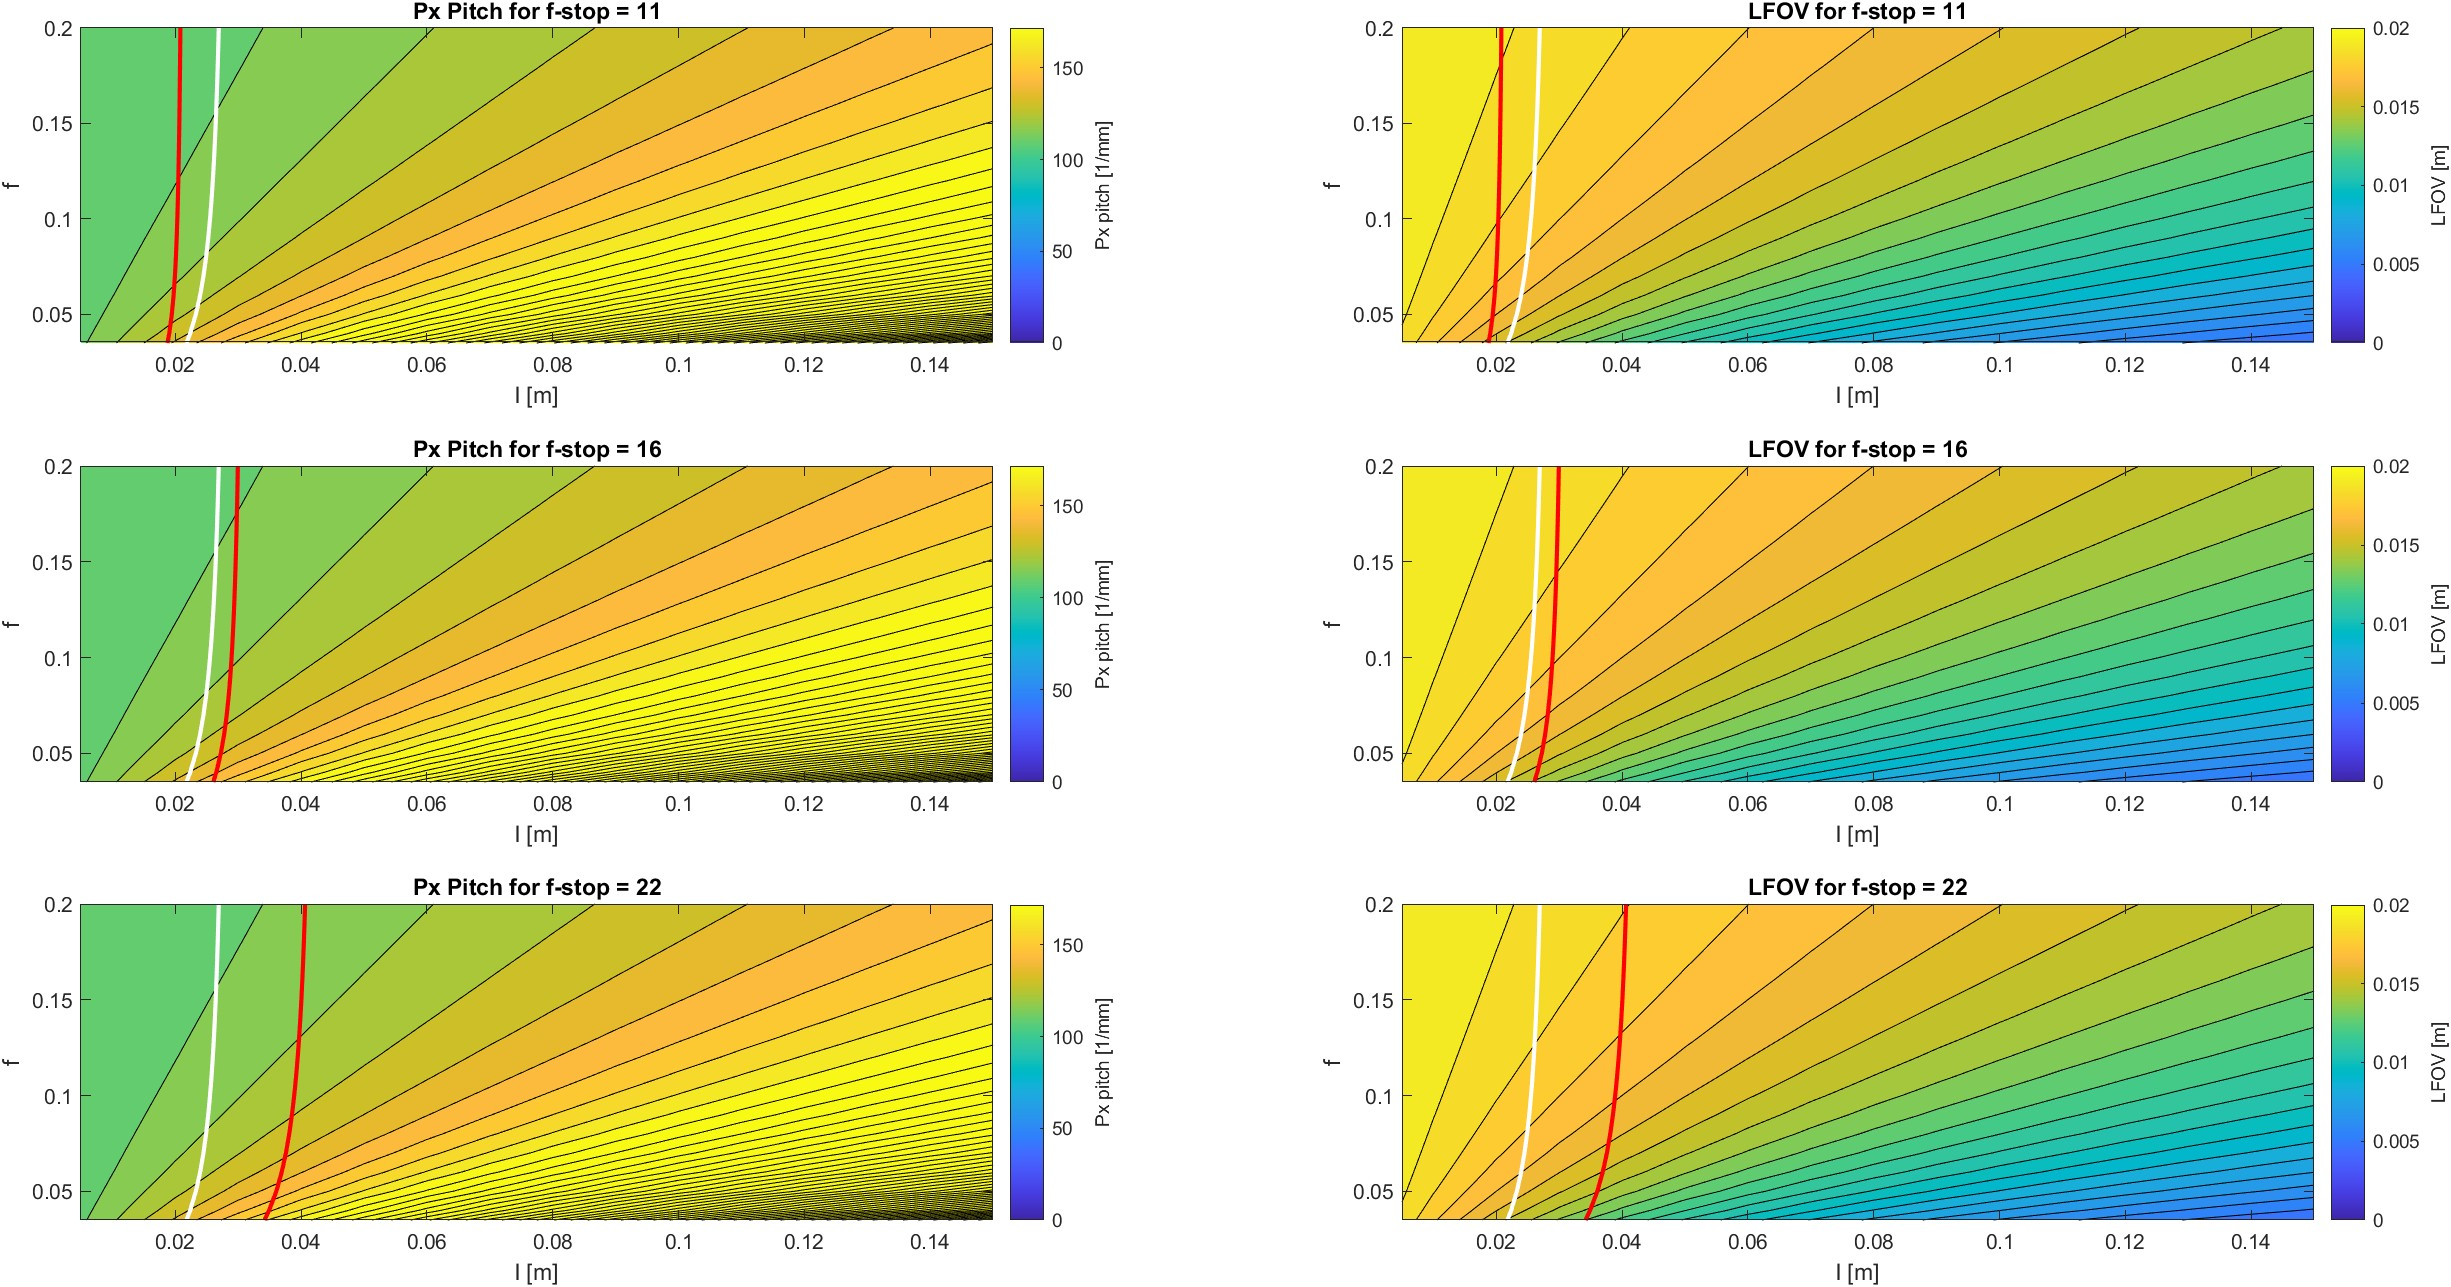
\includegraphics[width=1\textwidth]{figures/Px pitch and LFOV SBOS surf map.jpg}
    \caption{Surface maps of $\rho_{px}$ and $L_{FoV}$ for $f_\# \in $ [11,16,22],  $f \in $ (0.035,0.200), $l \in$ (0.005,0.15) and $L_{FoV_{obj}}=$ 2cm of a negative defocus setup, with the red isoline representing the points where $s_{min}$ =0.0004 m and the white line showing $S=0.02$.}
    \label{fig: Px pitch and LFOV surfmap SBOS}
\end{figure}

\section{Speckle size for positive defocus}
\label{section: Appendix speckle size BOS}

\par Figure \ref{fig: Delta s surfmap BOS} displays the speckle size of the positive defocus setup of Section \ref{subsection: Surface maps for BOS}. As in the negative defocus case, $\Delta s$ follows the trends of $M_{ag}$ through Equation \ref{equation: Rayleigh Limit}. It decreases with $l$ and increases with $f$, which is the inverse of the trend in Figure \ref{fig: Delta s design surfmap SBOS}. The smaller magnification of the positive defocus setup results in smaller speckles for the same $f_\#$, and both configurations converge to the same speckle size as $l$ approaches zero.

\begin{figure}[htbp]
    \centering
    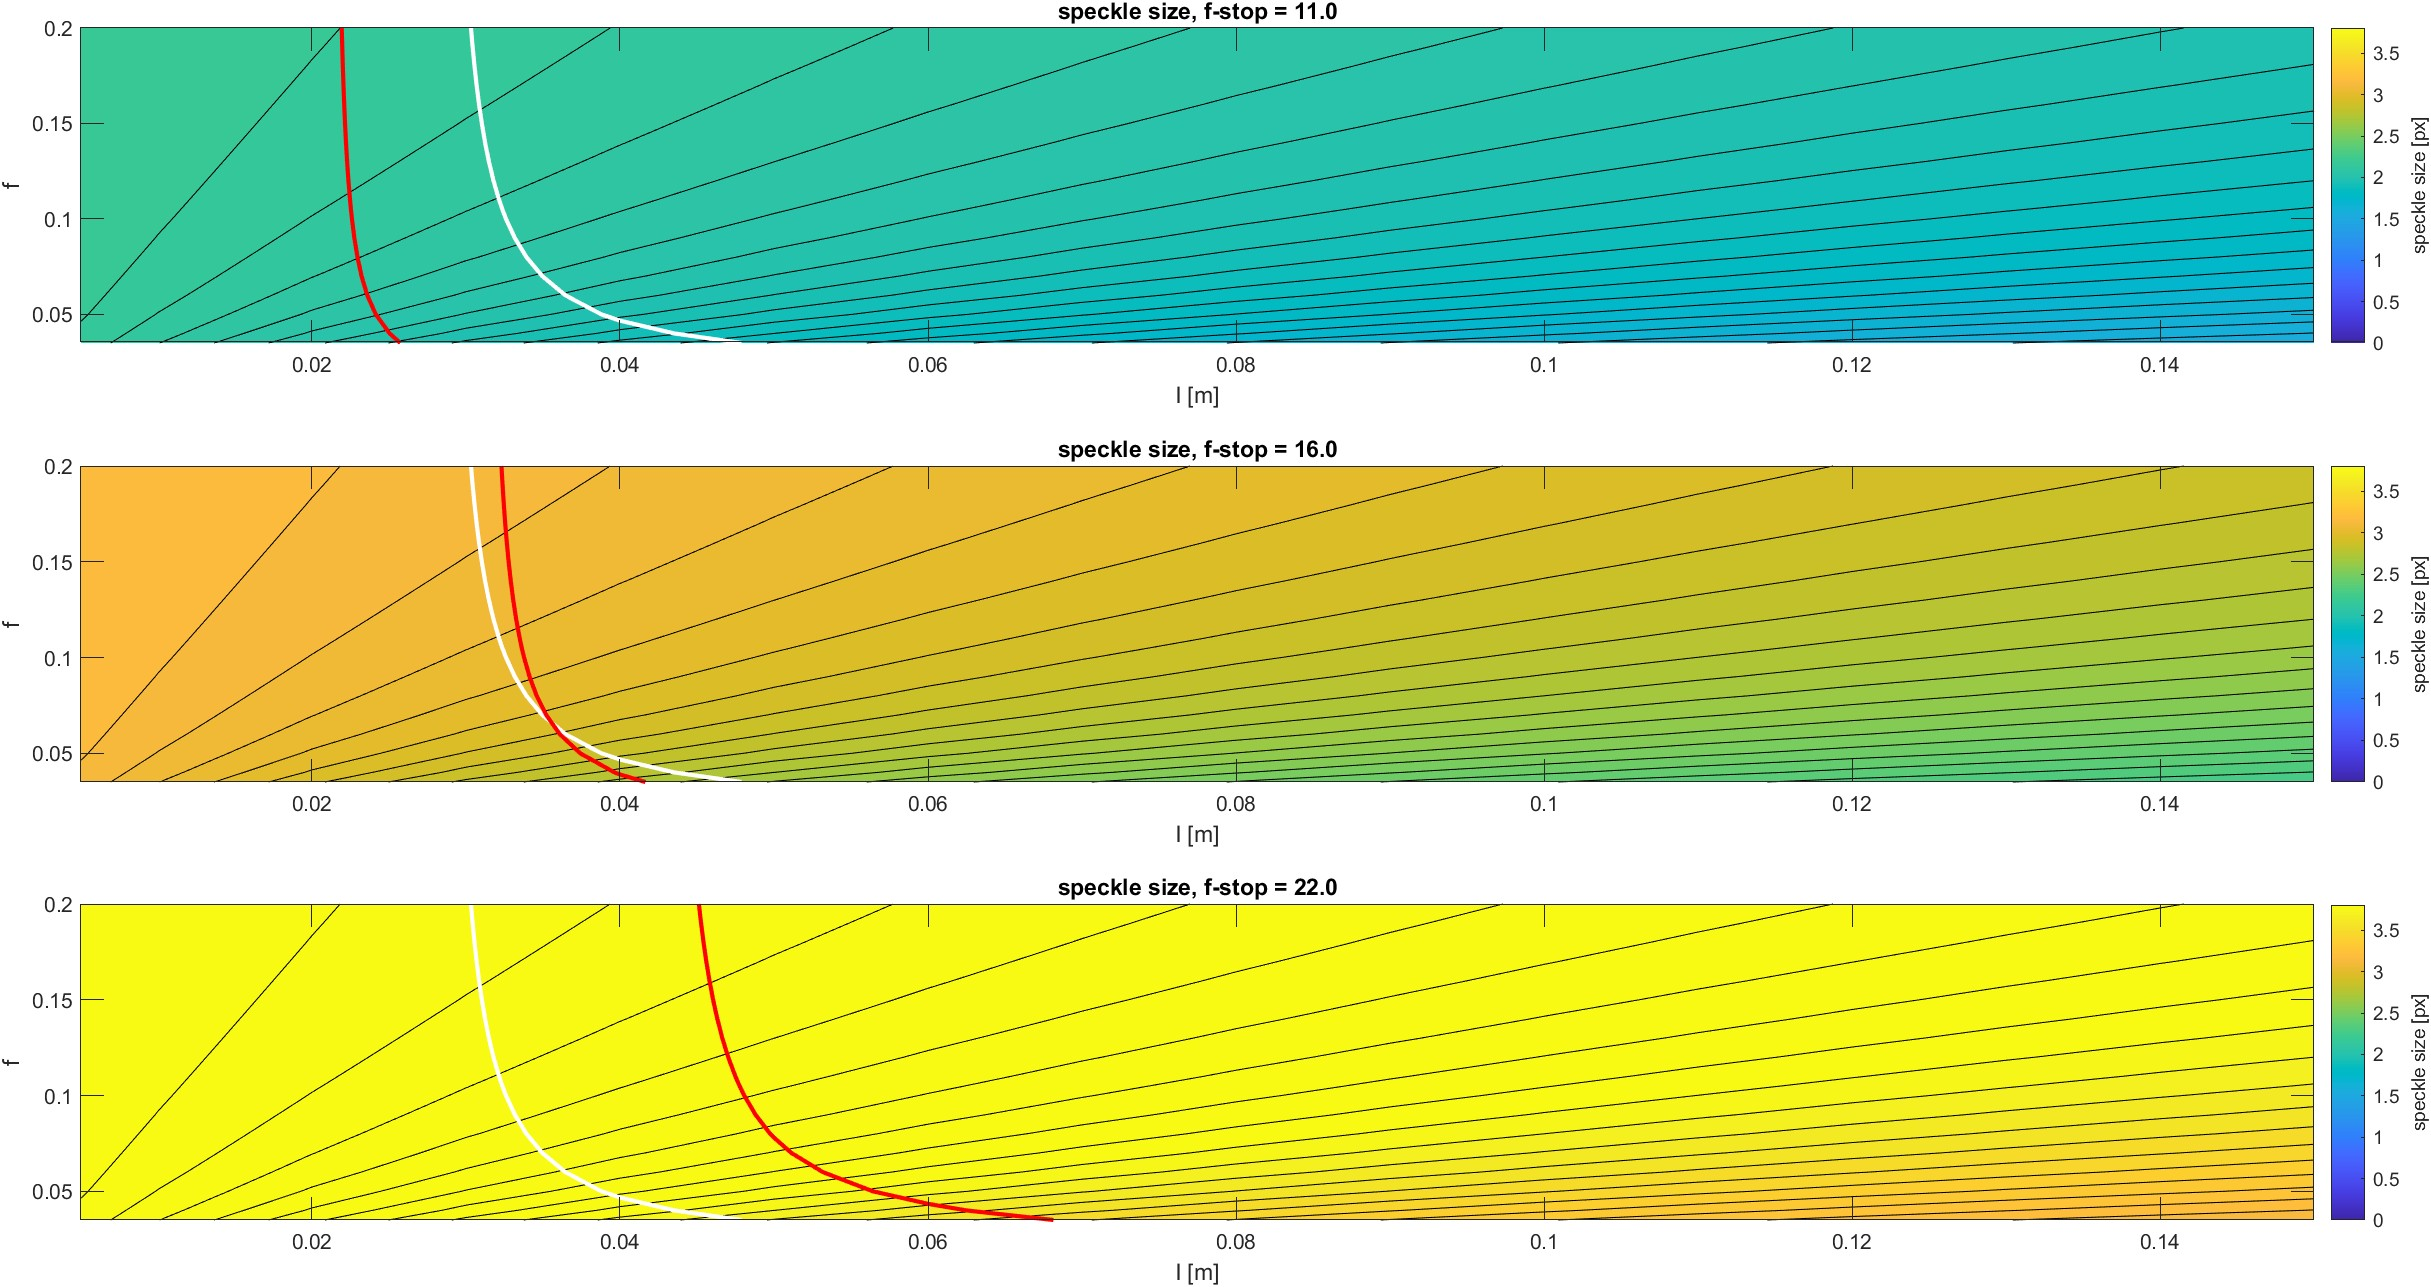
\includegraphics[width=1\textwidth]{figures/Speckle size surf map BOS.jpg}
    \caption{Surface maps of $\Delta s$ for $f_\# \in $ [11,16,22],  $f \in $ (0.035,0.200), $l \in$ (0.005,0.15) and $L_{FoV_{obj}}=$ 2cm of a positive defocus setup, with the red isoline representing the points where $s_{min}$ =0.0004 m and the white line showing $S=0.02$.}
    \label{fig: Delta s surfmap BOS}
\end{figure}

\section{Surface maps for a 7 cm field of view}
\label{section: Appendix 7cm FoV}

\par Figures \ref{fig: M,m,df surfmap SBOS 70mm} and \ref{fig: M,m,df surfmap BOS 70mm} display $M_{ag}$, $m$ and $d_f$ of the negative and positive defocus setups for $L_{FoV_{obj}} = 7$ cm, while Figure \ref{fig: Delta s surfmap 70mm} displays the respective speckle sizes. The trends are the same as the ones found for $L_{FoV_{obj}} = 2$ cm in Section \ref{section: Design Strategy}. The larger field of view, however, requires smaller magnifications and larger distances $m$ and $d_f$, which explains the smaller $S$ and $s_{min}$ discussed in Section \ref{subsection: Effects of FoV}. The smaller magnification also reduces the speckle size through Equation \ref{equation: Rayleigh Limit}.

\begin{figure}[htbp]
    \centering
    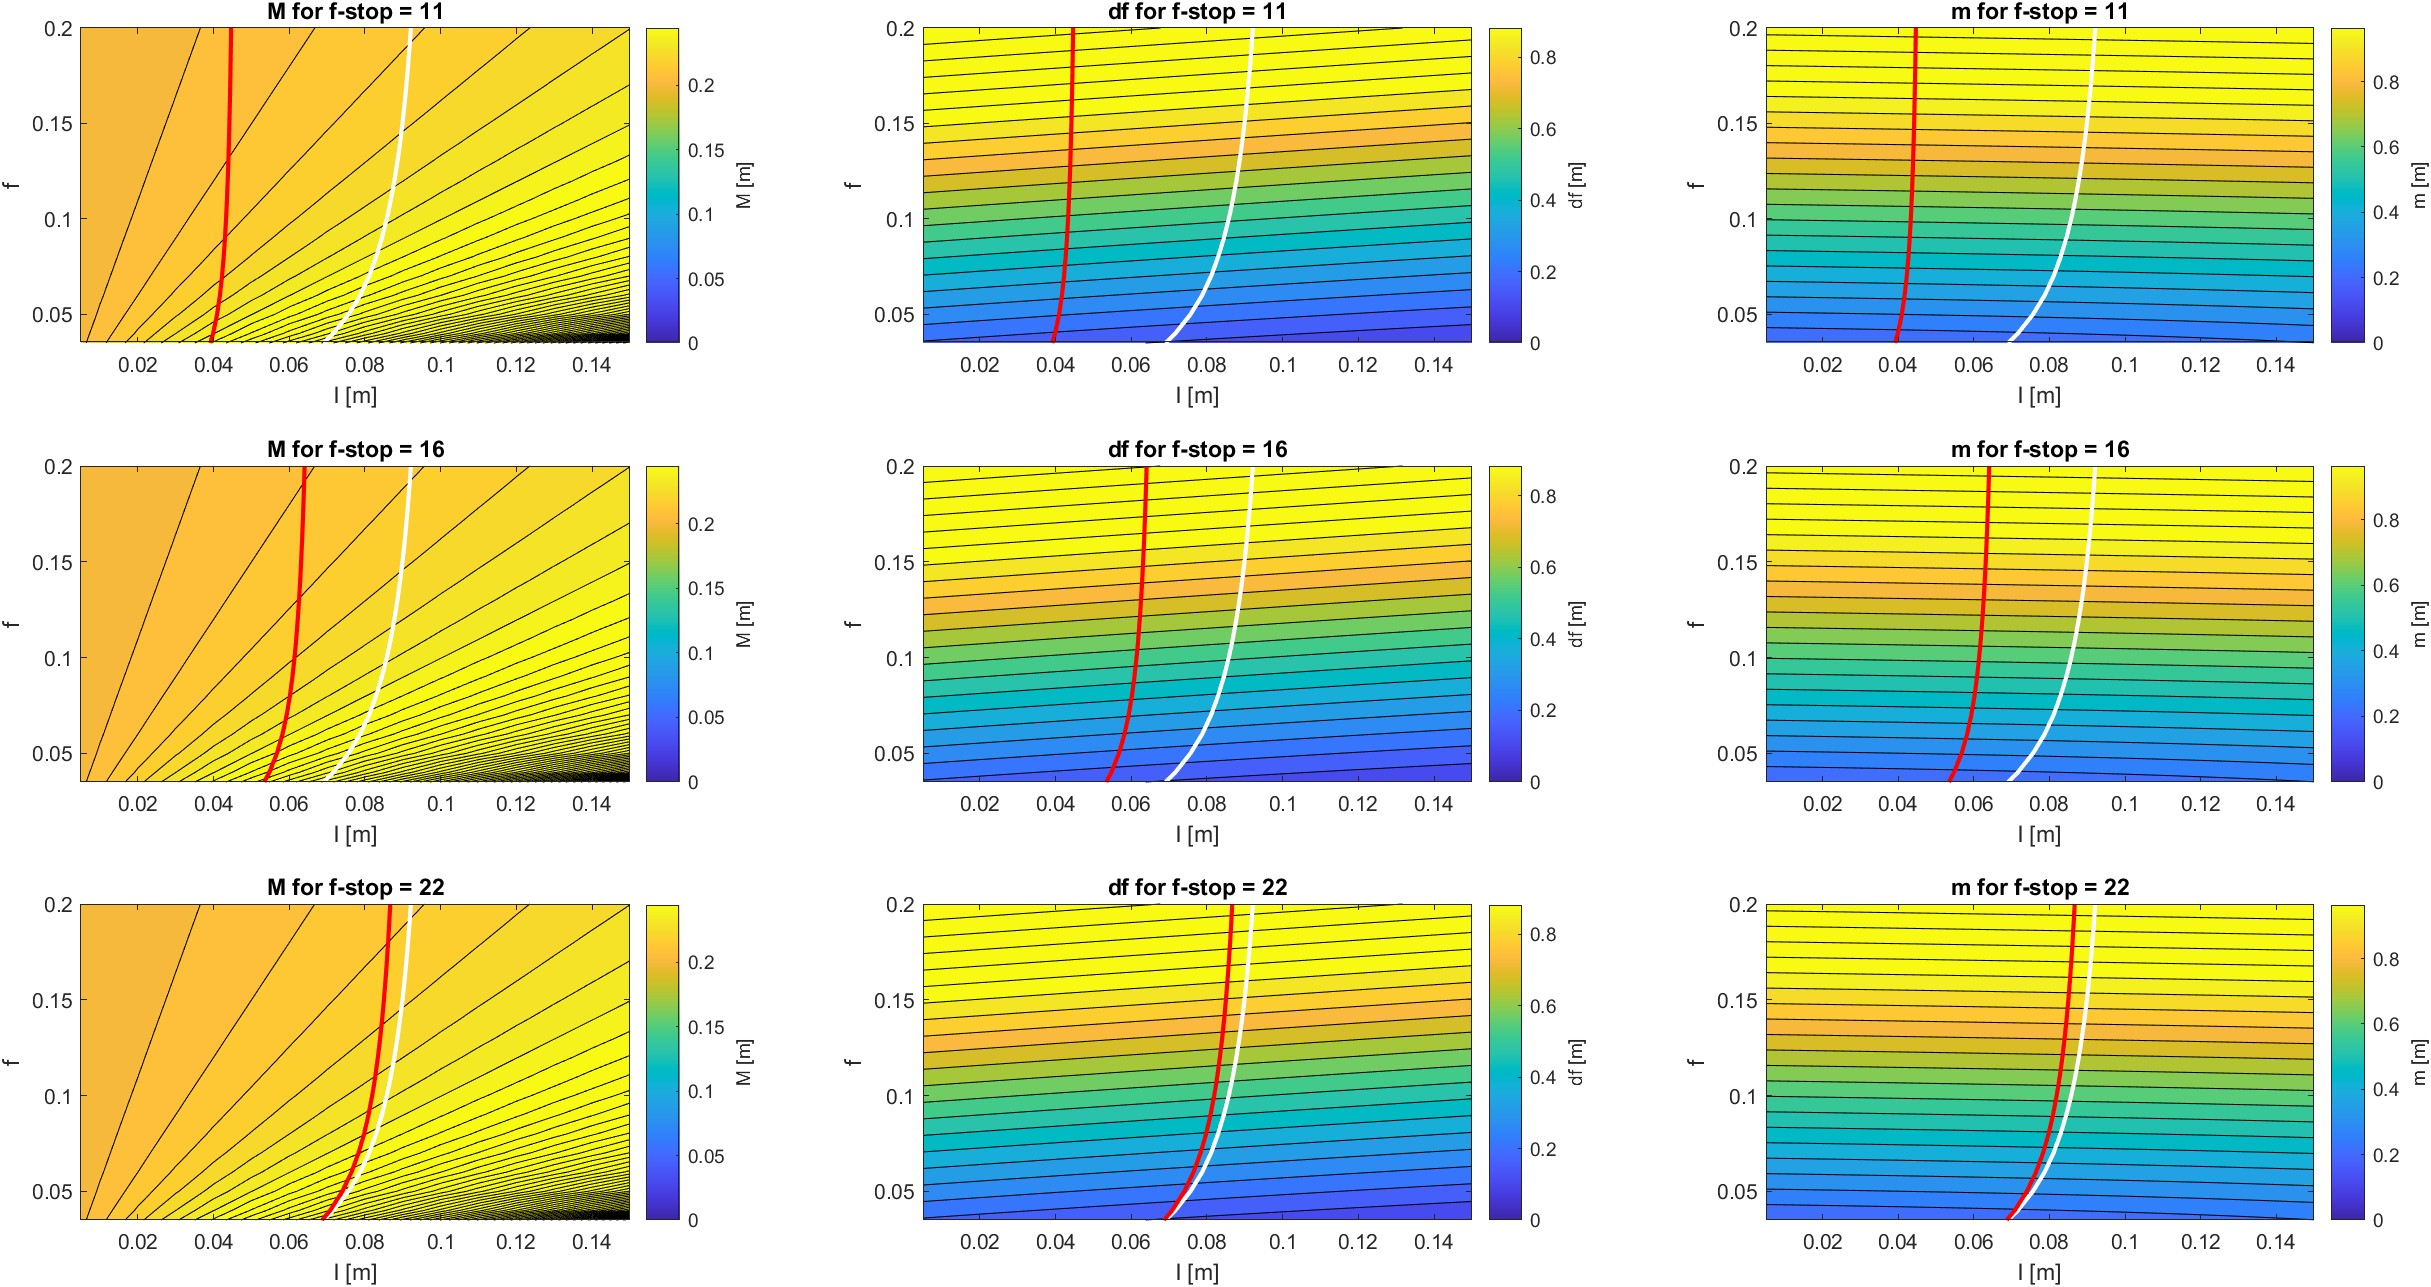
\includegraphics[width=1\textwidth]{figures/M,m,df surfmaps SBOS 70mm.jpg}
    \caption{Surface maps of $M_{ag}$, $m$ and $d_f$ for $f_\# \in $ [11,16,22],  $f \in $ (0.035,0.200), $l \in$ (0.005,0.15) and $L_{FoV_{obj}}=$ 7cm of a negative defocus setup, with the red isoline representing the points where $s_{min}$ =0.00035 m and the white line showing $S=0.02$.}
    \label{fig: M,m,df surfmap SBOS 70mm}
\end{figure}

\begin{figure}[htbp]
    \centering
    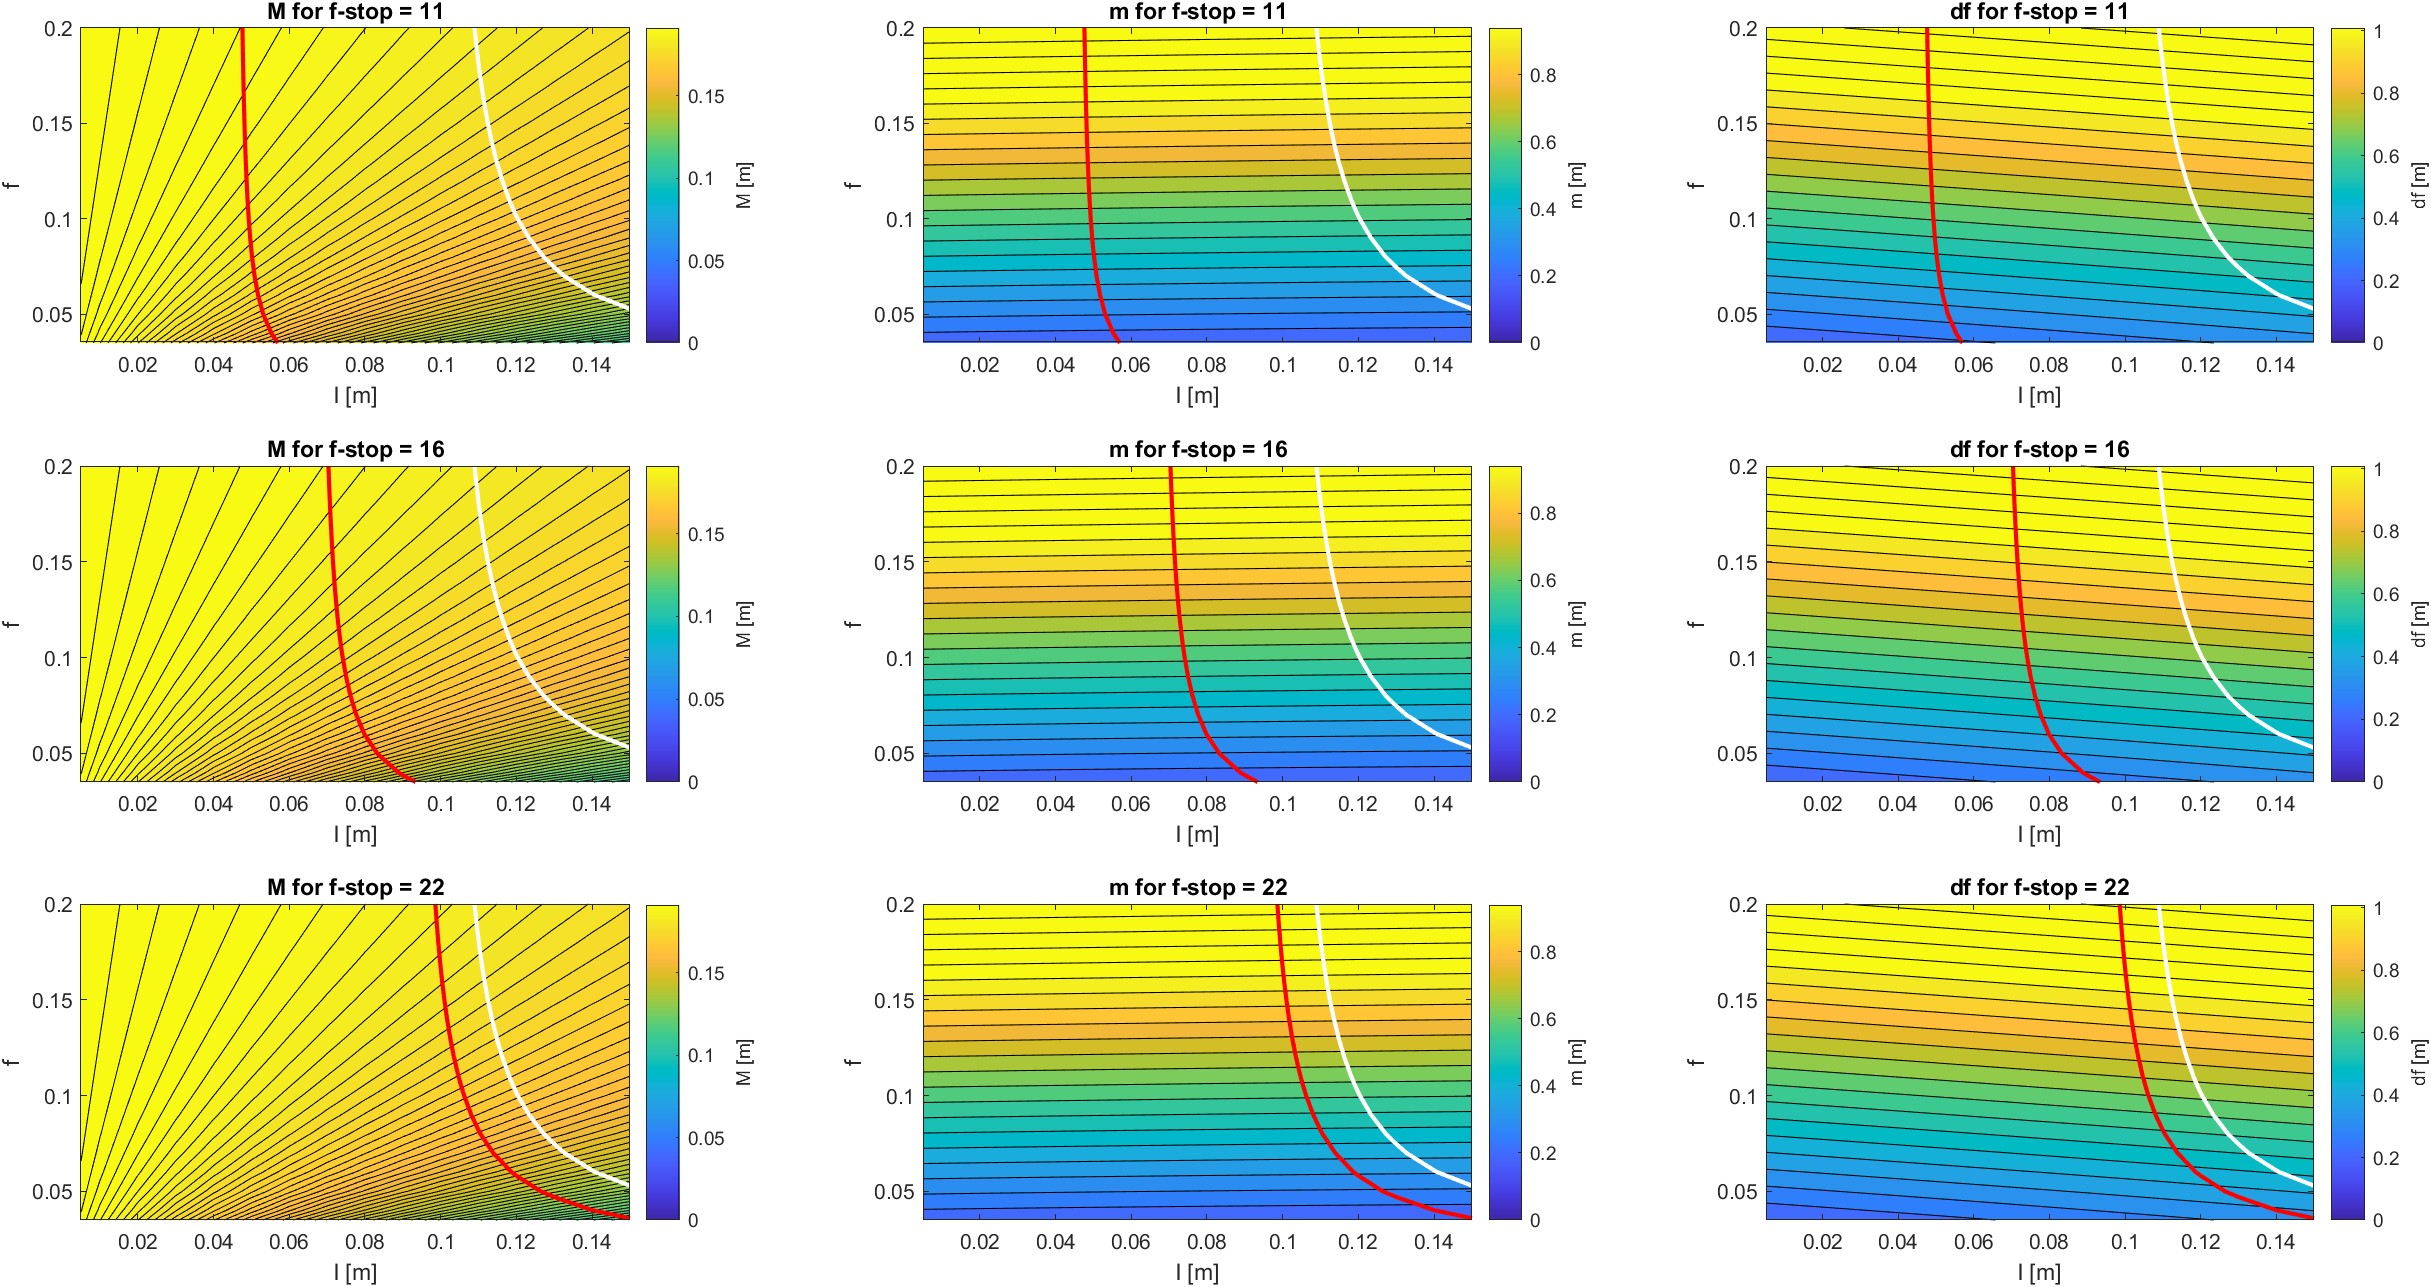
\includegraphics[width=1\textwidth]{figures/M,m,df surfmaps BOS 70mm.jpg}
    \caption{Surface maps of $M_{ag}$, $m$ and $d_f$ for $f_\# \in $ [11,16,22],  $f \in $ (0.035,0.200), $l \in$ (0.005,0.15) and $L_{FoV_{obj}}=$ 7cm of a positive defocus setup, with the red isoline representing the points where $s_{min}$ =0.00035 m and the white line showing $S=0.02$.}
    \label{fig: M,m,df surfmap BOS 70mm}
\end{figure}

\begin{figure}[htbp]
  \centering
  \begin{subfigure}{0.9\textwidth}
    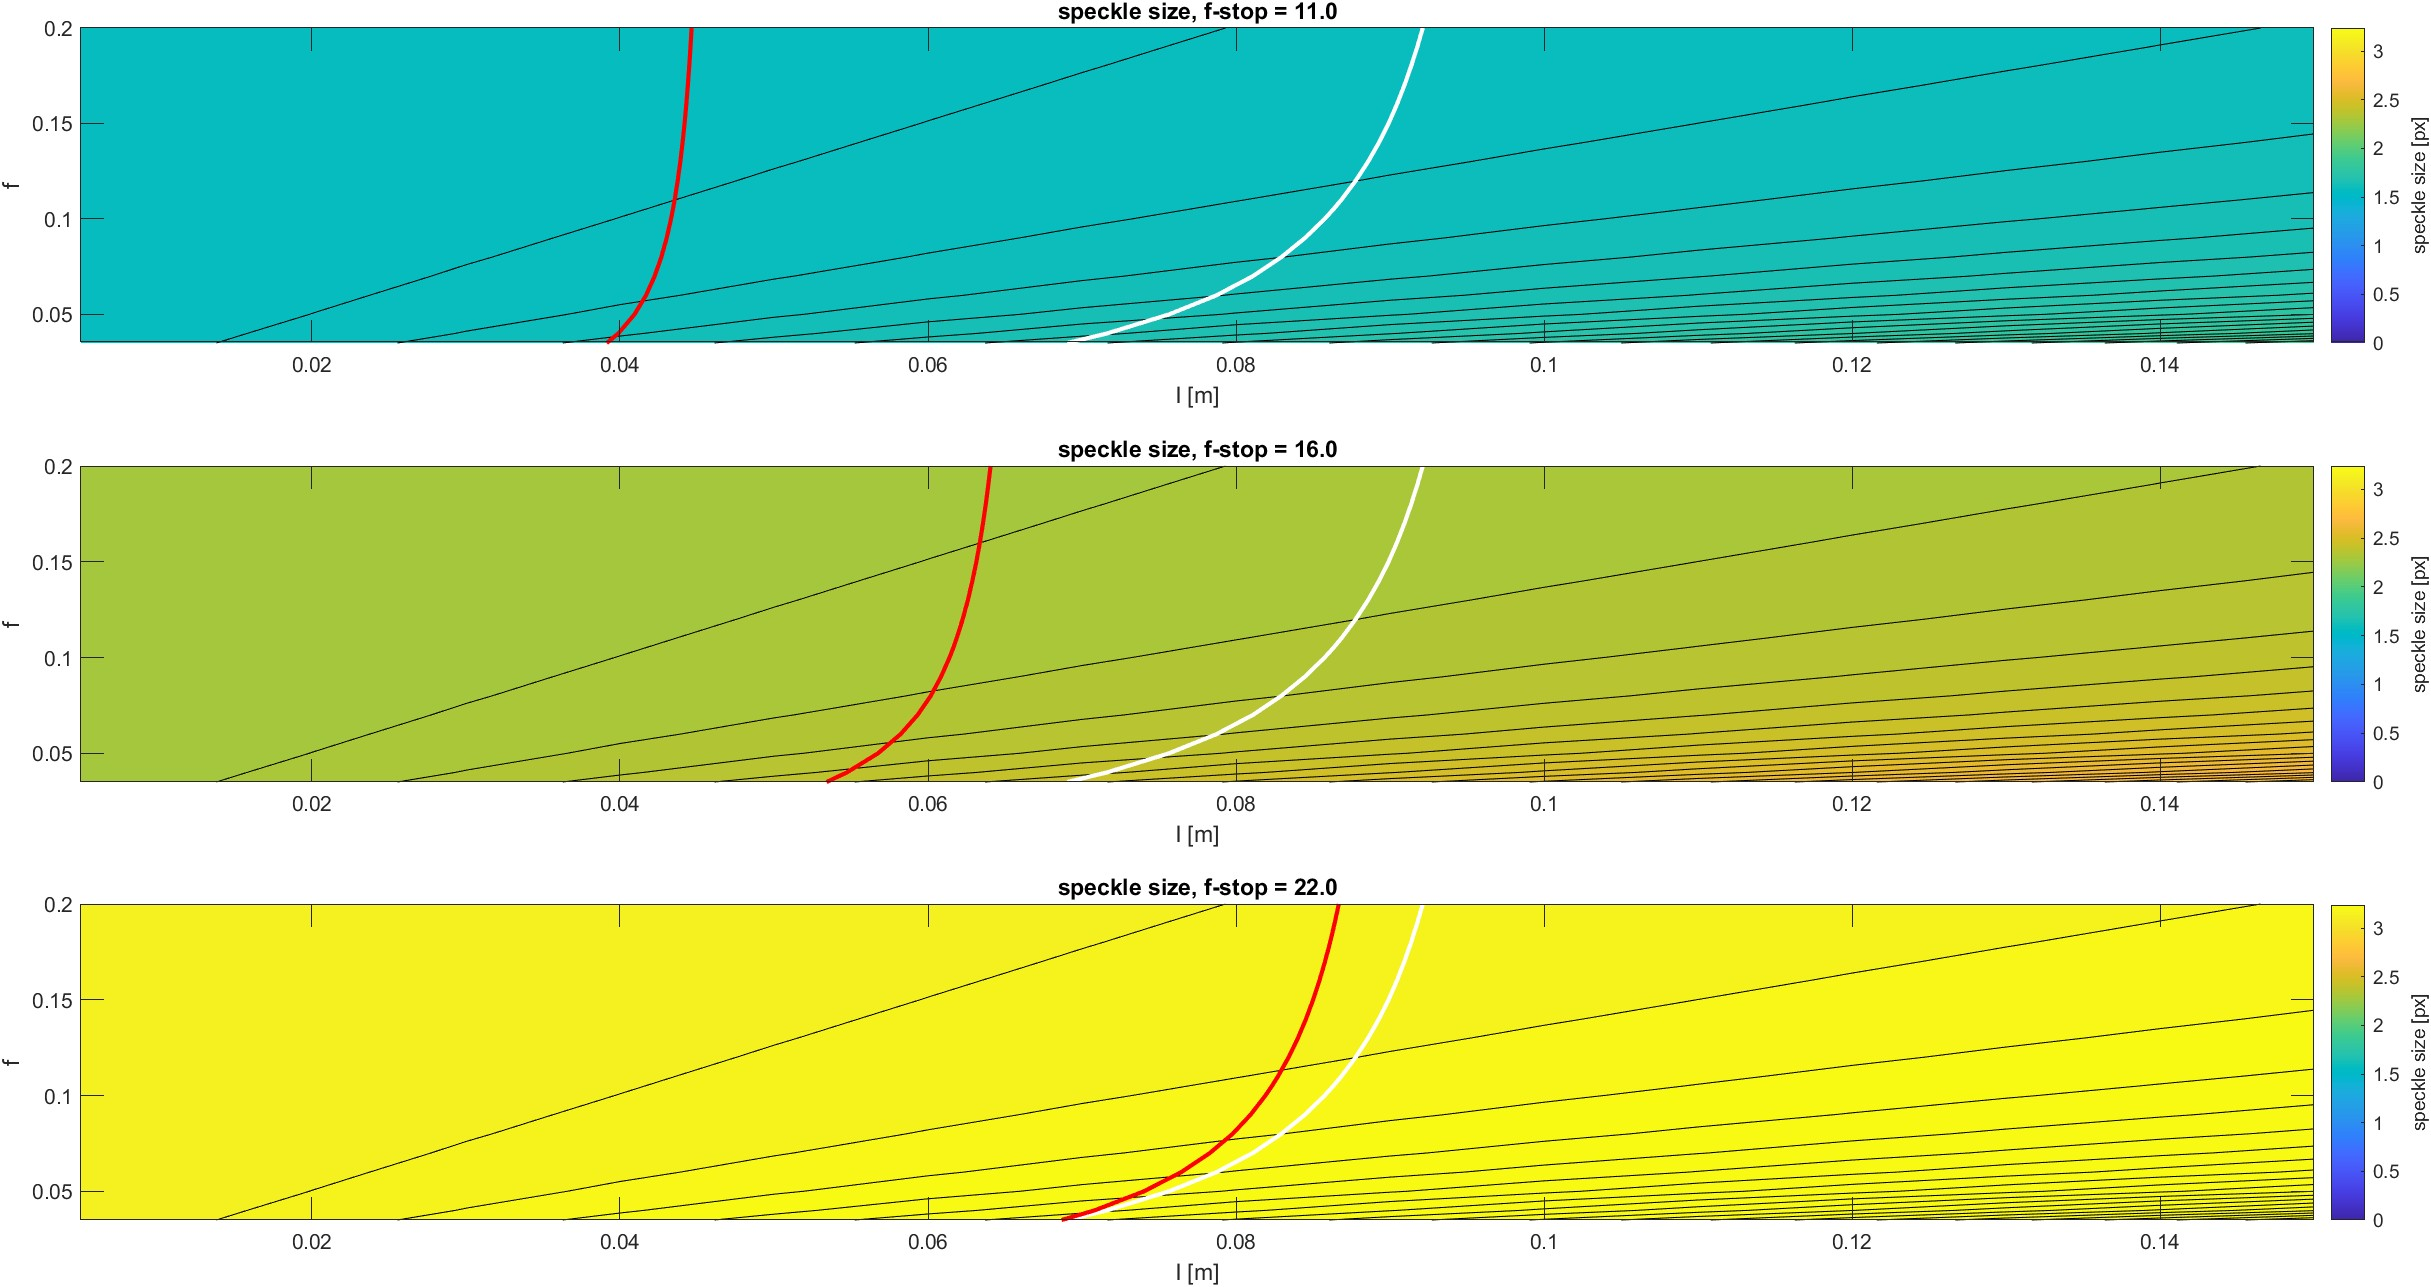
\includegraphics[width=\textwidth]{figures/Speckle size surf map SBOS 70mm.jpg}
    \caption{}
    \label{fig: Delta s surfmap SBOS 70mm}
  \end{subfigure}

  \begin{subfigure}{0.9\textwidth}
    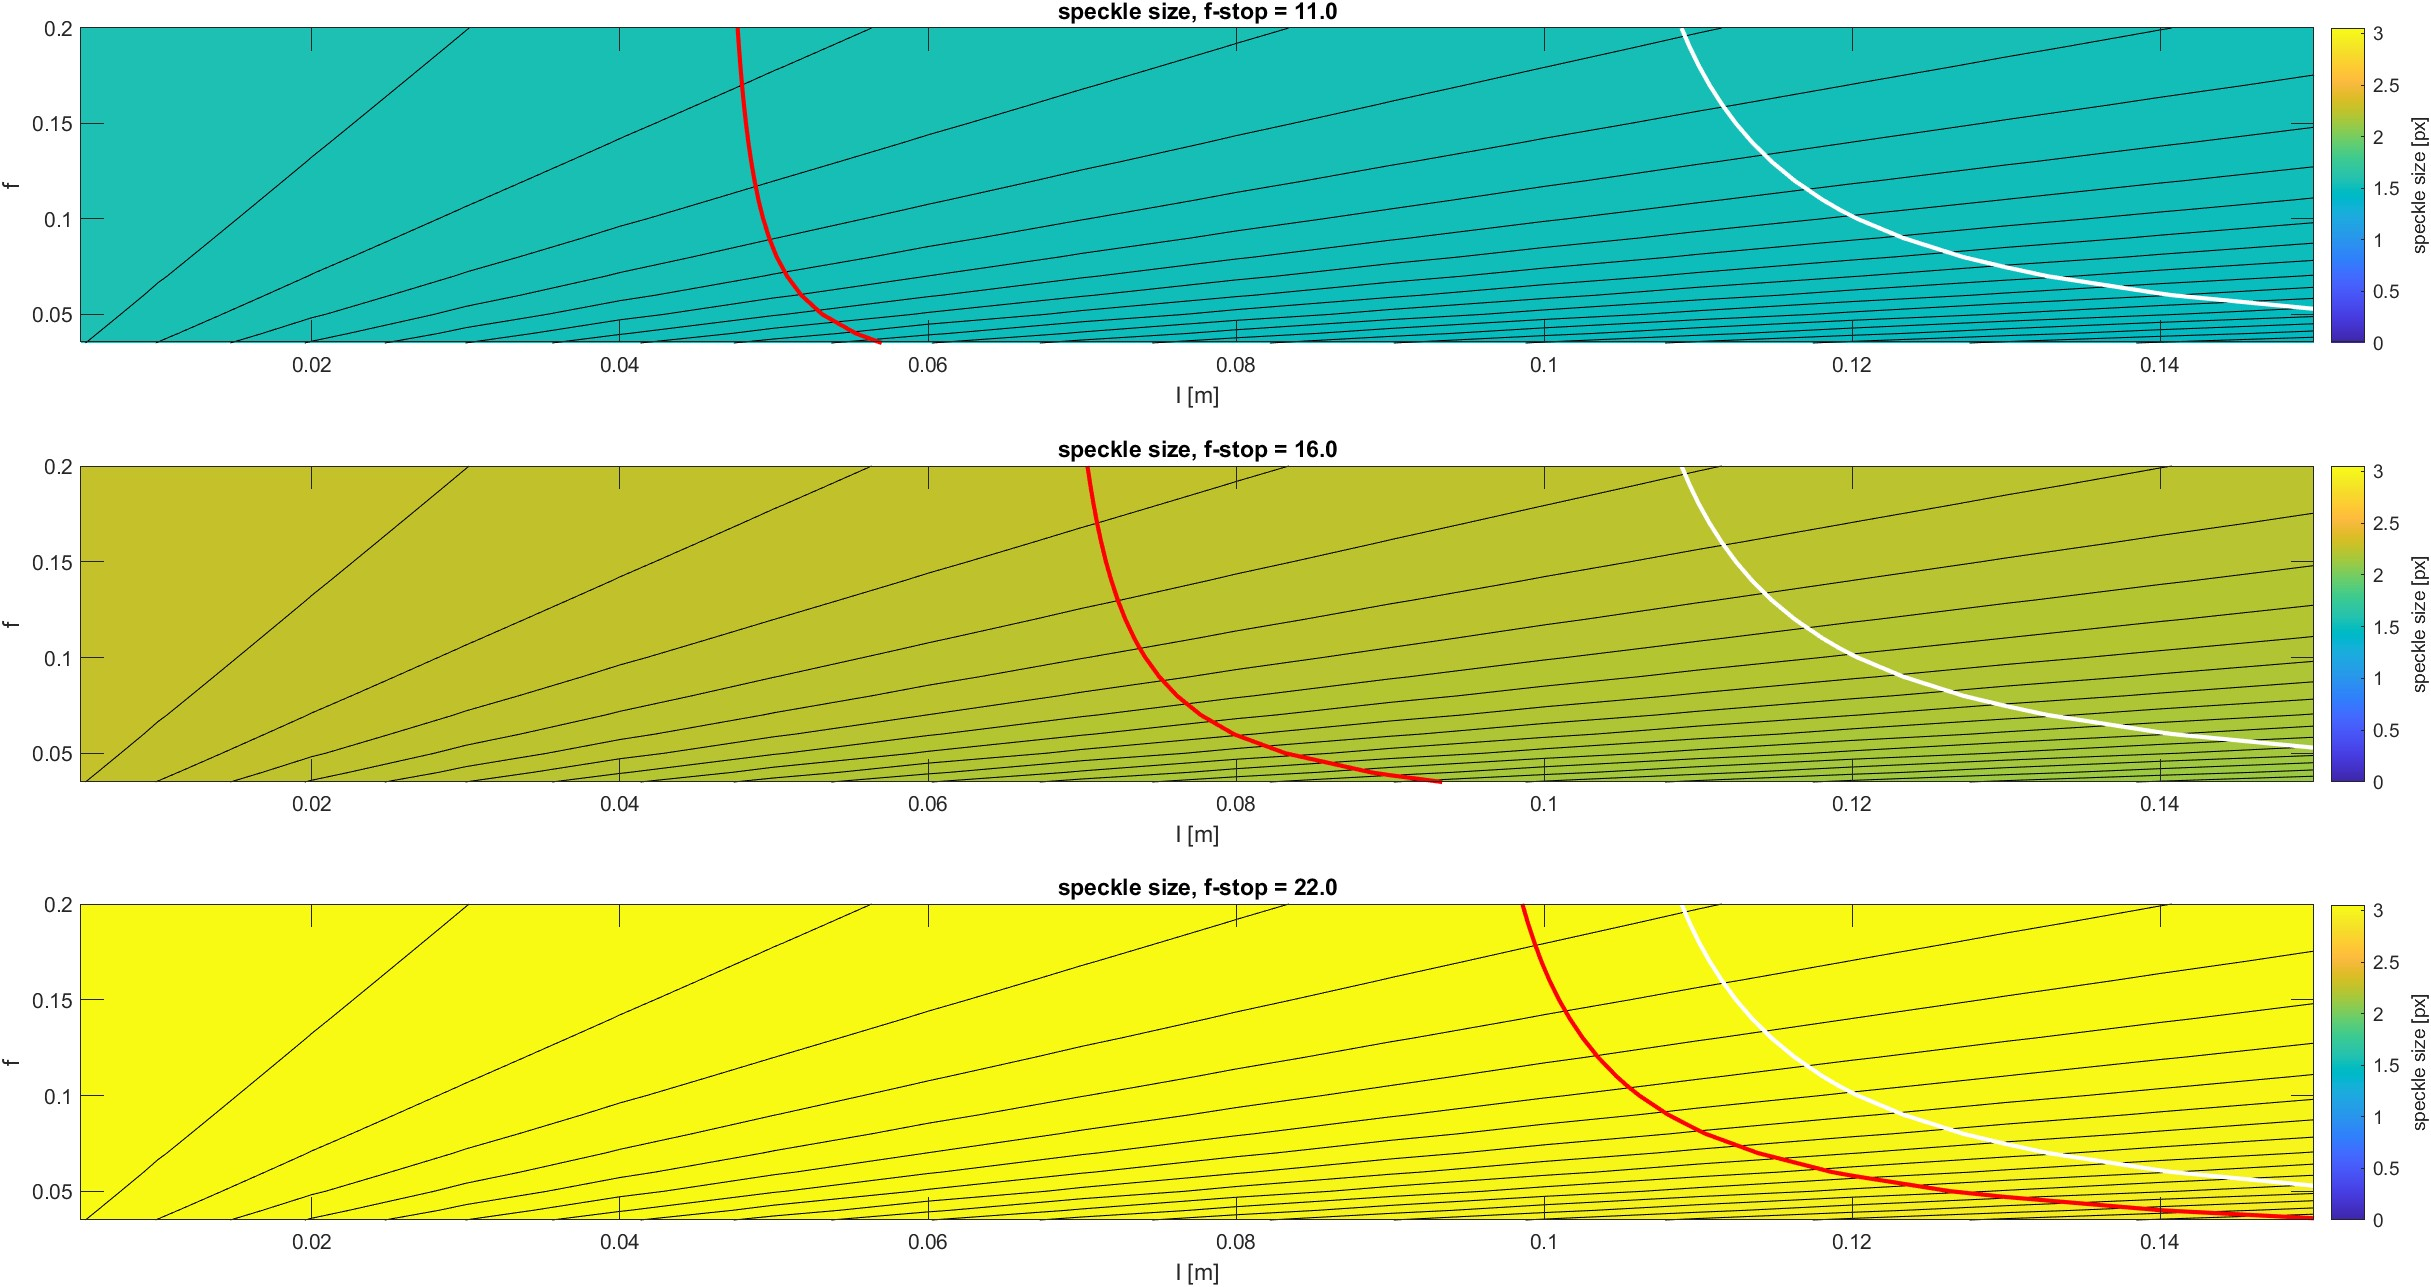
\includegraphics[width=\textwidth]{figures/Speckle size surf map BOS 70mm.jpg}
    \caption{}
    \label{fig: Delta s surfmap BOS 70mm}
  \end{subfigure}
  \caption{Surface maps of $\Delta s$ for $f_\# \in $ [11,16,22],  $f \in $ (0.035,0.200), $l \in$ (0.005,0.15) and $L_{FoV_{obj}}=$ 7cm of a negative defocus setup (a) and a positive defocus setup (b), with the red isoline representing the points where $s_{min}$ =0.00035 m and the white line showing $S=0.02$.}
  \label{fig: Delta s surfmap 70mm}
\end{figure}
